\documentclass{ximera}

\newcommand{\RR}{\mathbb R}
\renewcommand{\d}{\,d}
\newcommand{\dd}[2][]{\frac{d #1}{d #2}}
\renewcommand{\l}{\ell}
\newcommand{\ddx}{\frac{d}{dx}}
\newcommand{\dfn}{\textbf}
\newcommand{\eval}[1]{\bigg[ #1 \bigg]}


\author{Jason Miller}
\license{Creative Commons 3.0 By-bC}


\outcome{}

\begin{document}
\begin{exercise}


Consider the polar curve $r=\sin(2\theta)$. The graph is show below. 




\begin{image}  
  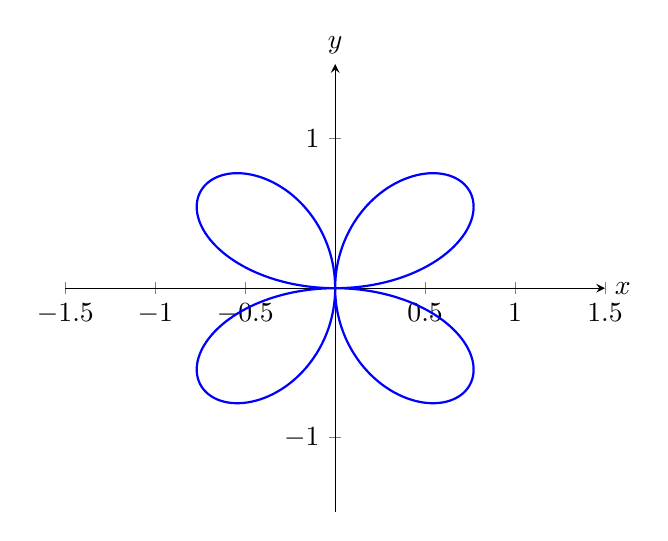
\begin{tikzpicture}  
    \begin{axis}[  
        xmin=-1.5,  
        xmax=1.5,  
        ymin=-1.5,  
        ymax=1.5,  
        axis lines=center,  
        xlabel=$x$,  
        ylabel=$y$,  
        every axis y label/.style={at=(current axis.above origin),anchor=south},  
        every axis x label/.style={at=(current axis.right of origin),anchor=west},  
      ]  
      \addplot[data cs=polar,blue,domain=0:360,samples=360,smooth, thick] (x,{sin(2*x)});
      \end{axis}  
  \end{tikzpicture}  
\end{image} 

We want to find tangent line to the curve when $\theta=\frac{\pi}{6}$. 

First find the point ( in Cartesian coordinates) on the curve $r=\sin(2\theta)$ when $\theta=\frac{\pi}{6}$. 
The point is $\left( \answer{ \frac{3}{4}},  \answer{ \frac{\sqrt{3}}{4}} \right)$. 

\begin{hint}

Recall that given the polar coordinates $(r,\theta)$ of a point, we can find the Cartesian coordinates $(x, y)$, using
\begin{align*}
x&=r\cos(\theta) \\
y&=r\sin(\theta)
\end{align*}

Since we want a point on the curve $r=1+\sin(\theta)$, we can substitute for $r$ and get:

\begin{align*}
x&=\answer{\sin(2\theta)\cos(\theta)} \\
y&=\answer{\sin(2\theta)\sin(\theta) }
\end{align*}

Now since we want the point corresponding to $\theta=\frac{\pi}{6}$ we have:


\begin{align*}
x&=\answer{ \frac{3}{4} } \\
y&=\answer{\frac{\sqrt{3}}{4}  }
\end{align*}

\end{hint}

\begin{exercise}

Find the slope of tangent line to the curve when $\theta=\frac{\pi}{6}$. 

The slope is $\answer{ \frac{5}{\sqrt{3}} }$.

\begin{hint}

Consider the formulas for changing from polar coordinates to Cartesian coordinates:

\begin{align*}
x&=r\cos(\theta) \\
y&=r\sin(\theta)
\end{align*}

Using the equation of our curve $r=1+\sin(\theta)$, we can substitute for $r$ to obtain:

\begin{align*}
x&=\answer{\sin(2\theta)\cos(\theta)} \\
y&=\answer{\sin(2\theta)\sin(\theta) }
\end{align*}

Note that we have expressed both the $x$ and $y$ coordinates of the points of the curve in terms of functions of a single parameter $\theta$. That means we have a parametric description for our curve in terms of $\theta$. 

Recall that for parametric equations 

\begin{align*}
x&=x(t) \\
y&=y(t)
\end{align*}

we could find the slope of the tangent line at a point corresponding to the parameter value $t$ by using 

$\dd[y]{x}=\frac{ y'(t)}{x'(t)}$


Since we have a parametric description of our curve in terms of $\theta$, 

\begin{align*}
x&=\answer{\sin(2\theta)\cos(\theta)} \\
y&=\answer{\sin(2\theta)\sin(\theta) }
\end{align*}

we use the same method for finding the slope. 

So we need to calculate

$\dd[y]{x}=\frac{ y'(\theta)}{x'(\theta)}$ and evaluate it at $\theta=\frac{\pi}{6}$. 

Calculating we get

\begin{align*}
x'(\theta)&=\answer{ 2\cos(2\theta)\cos(\theta)- \sin(2\theta)\sin(\theta)} \\
y'(\theta)&=\answer{ 2\cos(2\theta)\sin(\theta)+\sin(2\theta)\cos(\theta) }
\end{align*} 

Therefore $\dd[y]{x}$ evaluated when $\theta=\frac{\pi}{6}$ is $\answer{ \frac{5}{\sqrt{3}}  }$.


\end{hint}

\begin{exercise}

The tangent line to the curve when $\theta=\frac{\pi}{6}$ is given by 

$y-\answer{\frac{\sqrt{3}}{4}   }=\answer{ \frac{5}{\sqrt{3}}  }\left( x- \answer{  \frac{3}{4} }  \right)$. 

\begin{hint}


The point-slope formula for a line is give by $y-y_{0}=m(x-x_{0})$ where $m$ is the slope of the line and $(x_{0},y_{0})$ is a given point on the line. 
Since we want the tangent line to the curve $r=\sin(2\theta)$ when $\theta=\frac{\pi}{6}$, we need $(x_{0},y_{0})$ to be the point on the curve corresponding to the parameter value $\theta=\frac{\pi}{6}$ (we found this point earlier). The slope $m$ will be $\dd[y]{x}$ evaluated when $\theta=\frac{\pi}{6}$, which we also have previously calculated. 
The tangent line is shown below in red:

\begin{image}  
  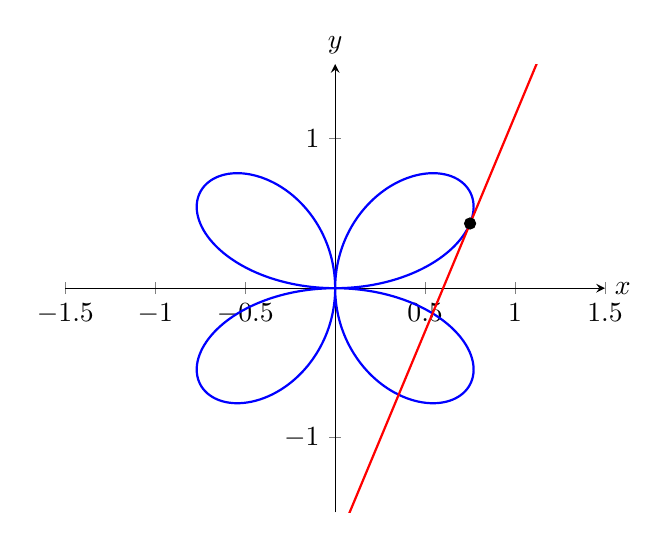
\begin{tikzpicture}  
    \begin{axis}[  
        xmin=-1.5,  
        xmax=1.5,  
        ymin=-1.5,  
        ymax=1.5,  
        axis lines=center,  
        xlabel=$x$,  
        ylabel=$y$,  
        every axis y label/.style={at=(current axis.above origin),anchor=south},  
        every axis x label/.style={at=(current axis.right of origin),anchor=west},  
      ]  
      \addplot[data cs=polar,blue,domain=0:360,samples=360,smooth, thick] (x,{sin(2*x)});
      \draw (axis cs:2,2.9) node { $r=\sin 2\theta$};
      \addplot[ red, domain=0:2, thick] {.433+2.887*(x-.75)};
     \addplot[only marks, mark=*] coordinates {(.75, .433)};
         \end{axis}  
  \end{tikzpicture}  
\end{image} 


\end{hint}

\end{exercise}
\end{exercise}
\end{exercise}
\end{document}
